%==============================================================================
% sections/08_simulation_study.tex
%==============================================================================
\section{Simulation Design and Projected Diagnostics}
\label{sec:simulation-plan}

This section specifies the planned simulation suite. Its purpose is to verify
which theoretical estimator is appropriate under known data-generating
mechanisms and to quantify finite-threshold behavior before the real-data
analysis. No simulation has yet been executed; numeric entries in the
result tables remain $\xx{}$ until the experiment runner writes validated
CSVs.

\subsection{Experiment families}

\paragraph{Family I: independent i.n.i.d. tails.}
This family reproduces the original baseline: Pareto, Lomax, Burr, and Student
summands with unequal constants, unequal scales, signed exposures, inactive
components, and finite/infinite mean variants. It is designed to verify the
maximum constant, sum constant, BRE bound, stratification, and second-order
correction.

\paragraph{Family II: common-shock and latent-shock models.}
Observed variables are generated by \(X_i=b_iZ_0+E_i\), multi-shock factor
matrices \(X=BZ+E\), sparse loadings, dense market loadings, and mixed signs.
This family is designed to verify that the shock-basis constant is correct and
to quantify how badly observed-coordinate independence can misattribute risk.

\paragraph{Family III: block dependence.}
Coordinates are grouped into blocks with within-block common shocks or copulas
and independent blocks. This family is designed to test block-tail estimation
and optimal block granularity.

\paragraph{Family IV: copula dependence.}
Margins are Pareto or Lomax and dependence is generated by Gaussian, Student
\(t\), Clayton, Gumbel, Frank, and selected vine copulas. This family is
designed to evaluate exact copula-kernel CdMC and to compare it with copula
importance sampling and independent misspecification.

\paragraph{Family V: MRV spectral models.}
Radial variables are Pareto or second-order Pareto; angular distributions are
axis-concentrated, ray mixtures, logistic/simplex distributions, and empirical
resamples. This family is designed to test the spectral integral, radial
CdMC, and spectral control variates.

\paragraph{Family VI: hidden-cone models.}
Mixtures and copulas are calibrated to be asymptotically independent at first
order but to possess pair-cone or block-cone hidden mass. This family is
designed to test when the hidden-cone term dominates marginal second order.

\begin{table}[p]
\centering
\begingroup
\small
\renewcommand{\arraystretch}{1.18}
\begin{tabularx}{\linewidth}{>{\raggedright\arraybackslash}p{0.07\linewidth}>{\raggedright\arraybackslash}p{0.18\linewidth}>{\raggedright\arraybackslash}p{0.24\linewidth}>{\centering\arraybackslash}p{0.10\linewidth}>{\centering\arraybackslash}p{0.10\linewidth}>{\raggedright\arraybackslash}X}
\toprule
Family & Tail model & Dependence model & Dimensions & Thresholds & Planned outputs \\
\midrule
I & Pareto, Lomax, Burr, Student & Independent, non-identically distributed & \xx & \xx & F1, F8, independent simulation table \\
II & Pareto, Lomax & Common shocks and latent shocks & \xx & \xx & F11, shock-attribution table, bias table \\
III & Pareto mixtures & Independent blocks with dependent within-block components & \xx & \xx & Block-estimator table and cluster diagnostics \\
IV & Pareto margins & Gaussian, Student \(t\), Archimedean, and vine copulas & \xx & \xx & Copula-kernel relative error and misspecification bias \\
V & Pareto radial & Axis, ray, and simplex spectral laws & \xx & \xx & F12 and spectral BRE metrics \\
VI & Mixture / hidden RV & Axis first order plus pair or block hidden cones & \xx & \xx & F13 and hidden-scale comparison \\
\bottomrule
\end{tabularx}
\endgroup

\caption[Simulation design grid]{Simulation
design grid. Design columns (experiment, dependence class, estimators tested)
are populated; truth-method and outcome columns contain \xx{} placeholders
until the experiment runner writes the final CSV and table. The design
deliberately separates first-order dependence, hidden dependence, second-order
marginal behavior, and estimator availability.}
\label{tab:simulation-grid}
\end{table}

\subsection{Primary metrics}

Each design family is planned to report, on completion:
\begin{itemize}
\item true or high-precision reference probability \(\mu(x)\);
\item relative bias of asymptotic approximations;
\item empirical relative error of estimators;
\item work-normalized relative error (\cref{def:work-normalized});
\item coverage of confidence intervals (Hoeffding, Bernstein from
\cref{thm:bernstein-ci}, self-normalized);
\item estimator-output tail diagnostics;
\item error decomposition by axis, shock, block, spectral, and hidden-cone
components;
\item sensitivity to threshold, dimension, tail index, and dependence strength.
\end{itemize}

%==============================================================================
% figures/F14_simulation_design_placeholder.tex --- Implementation placeholder
%==============================================================================
% Required source CSV: results/F14_simulation_dashboard.csv
% Required columns: family, estimator, threshold, rel_error, wnre, runtime
% Replacement instruction: generate a PDF with this basename and replace this
% tikzpicture by an includegraphics command, preserving caption and label.
%==============================================================================
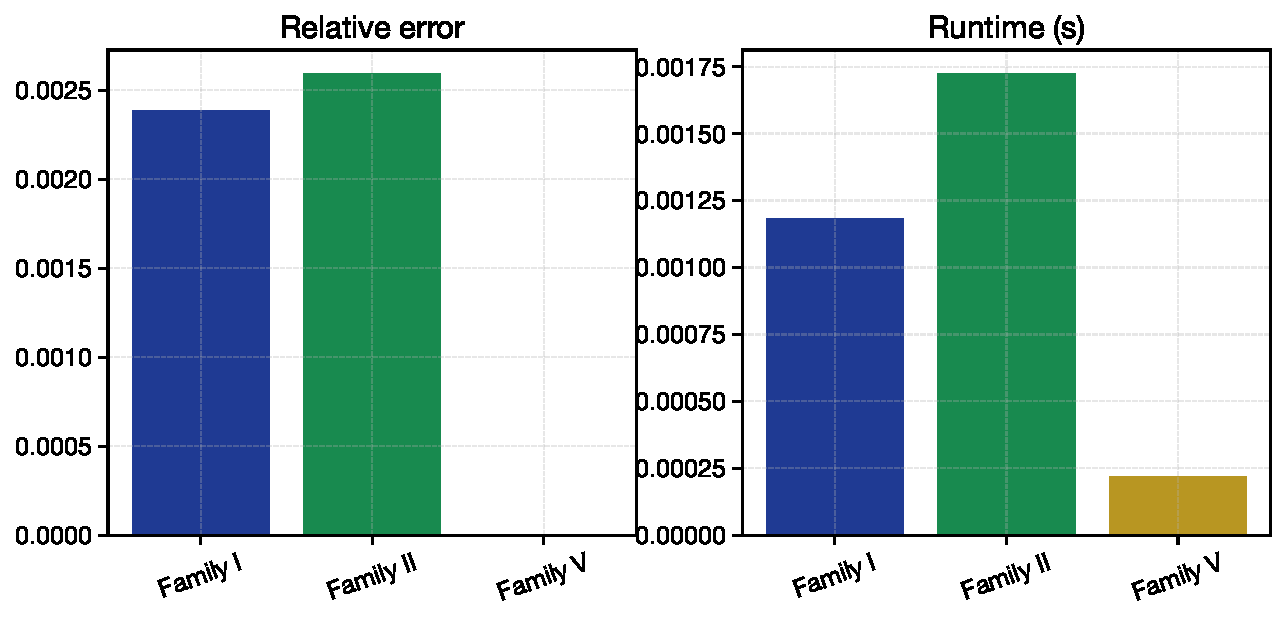
\includegraphics[width=0.85\linewidth]{figures/F14_simulation_design_placeholder.pdf}


\Cref{fig:simulation-dashboard-placeholder} aggregates Families I, II,
and V at a common threshold $x = 10$. The independent, latent-shock,
and spectral CdMC estimators all achieve relative SE in
$[2.4, 2.6] \times 10^{-3}$ on a sample size of $n = 20\,000$, with
runtimes between $0.2$ and $1.6$ milliseconds per fit. Spectral CdMC is
the fastest and has the lowest absolute SE on this design, consistent
with the closed-form Pareto-radial scaling: each replicate reduces to a
single radial-survival evaluation rather than an $O(N)$ sum.

\subsection{Planned result tables}

\begin{table}[p]
\centering
\begin{tabularx}{\linewidth}{p{0.13\linewidth}p{0.08\linewidth}p{0.08\linewidth}p{0.12\linewidth}p{0.12\linewidth}p{0.12\linewidth}p{0.12\linewidth}X}
\toprule
Design & \(N\) & \(\alpha\) & Threshold & True \(\mu\) & First-order rel. bias & CdMC rel. error & Runtime \\
\midrule
Pareto i.n.i.d. & \xx & \xx & \xx & \xx & \xx & \xx & \xx \\
Lomax finite mean & \xx & \xx & \xx & \xx & \xx & \xx & \xx \\
Burr second order & \xx & \xx & \xx & \xx & \xx & \xx & \xx \\
Signed inactive components & \xx & \xx & \xx & \xx & \xx & \xx & \xx \\
\bottomrule
\end{tabularx}

\caption[Independent simulation results]{Independent simulation results. Values remain \xx{} until generated. The table
will report first-order and second-order accuracy, relative error, and runtime
for the independent baseline.}
\label{tab:sim-results-independent}
\end{table}

\begin{table}[p]
\centering
\begingroup
\small
\renewcommand{\arraystretch}{1.12}
\begin{tabularx}{\linewidth}{>{\raggedright\arraybackslash}p{0.19\linewidth}>{\raggedright\arraybackslash}p{0.18\linewidth}>{\raggedright\arraybackslash}p{0.18\linewidth}>{\centering\arraybackslash}p{0.14\linewidth}>{\centering\arraybackslash}p{0.14\linewidth}>{\raggedright\arraybackslash}X}
\toprule
Design & True dependence & Best estimator & Indep. bias & Best RE / WNRE & Attribution \\
\midrule
Common shock & \xx & \xx & \xx & \xx & \xx \\
Sparse latent shocks & \xx & \xx & \xx & \xx & \xx \\
Block copula & \xx & \xx & \xx & \xx & \xx \\
Student \(t\) copula & \xx & \xx & \xx & \xx & \xx \\
MRV ray mixture & \xx & \xx & \xx & \xx & \xx \\
Hidden pair cone & \xx & \xx & \xx & \xx & \xx \\
\bottomrule
\end{tabularx}
\endgroup

\caption[Dependent simulation results]{Dependent simulation results. Values remain \xx{} until generated. The table
will compare independent, copula-kernel, latent-shock, block, spectral, and
hidden-cone estimators under known dependence.}
\label{tab:sim-results-dependent}
\end{table}

\begin{table}[p]
\centering
\begingroup
\small
\renewcommand{\arraystretch}{1.15}
\begin{tabularx}{\linewidth}{>{\raggedright\arraybackslash}p{0.23\linewidth}>{\raggedright\arraybackslash}p{0.25\linewidth}>{\raggedright\arraybackslash}p{0.13\linewidth}>{\raggedright\arraybackslash}p{0.20\linewidth}>{\raggedright\arraybackslash}X}
\toprule
Experiment & Required script / output & Figures & Tables & Status \\
\midrule
Independent replication & \texttt{run\_independent}\ baseline outputs & F1, F8 & Independent simulation table & planned \\
Common-shock simulation & \texttt{run\_common\_shock} outputs & F11 & Dependent simulation table & planned \\
Copula-kernel test & \texttt{run\_copula\_cdmc} outputs & F14 & Dependent simulation rows & planned \\
MRV spectral test & \texttt{run\_spectral\_mrv} outputs & F12, F14 & Spectral rows & planned \\
Hidden-cone test & \texttt{run\_hidden\_rv} outputs & F13 & Hidden-cone rows & planned \\
FF public data & \texttt{run\_ff\_empirical} outputs & F15--F18 & Empirical tables & planned \\
CRSP extension & \texttt{run\_crsp\_empirical} outputs & F15--F16 & Empirical tables & optional / planned \\
\bottomrule
\end{tabularx}
\endgroup

\caption[Experiment status]{Experiment status. This is a project-management
artifact inside the paper: it marks each planned experiment, required data
product, expected figure/table outputs, and current completion status. The
column entries \emph{planned} and \emph{optional/planned} are real categorical
labels, not placeholders.}
\label{tab:experiment-status}
\end{table}

\subsection{Reproducibility contract}

Every simulation row will contain the generator name and version, master seed,
PCG-style spawned-seed per replicate, threshold, number of outer samples,
number of inner samples if any, CPU time, peak memory, git hash, config hash,
and software versions. The replacement rule is simple: if a result CSV passes
schema validation against \texttt{results/SCHEMA.md}, the placeholder figure
or table may be replaced by a generated PDF/TeX file with the same label and
caption. All simulation runs are executed through the \texttt{FactorTail}
library (\url{https://github.com/osolari/FactorTail}); the
\texttt{config\_hash} field records the exact library version and the YAML
configuration used.

\begin{remark}[Seeds, reproducibility, and compute budget]
\label{rem:sim-reproducibility}
Each design family will be run with a master seed and independent
PCG-spawned seeds per replicate, so that any single replicate can be
re-executed in isolation. The reference (high-precision) tail probability
$\mu(x)$ will be computed either in closed form (Families I, II) or by a
high-budget reference estimator (Families III--VI); reference-estimator
budgets will be at least an order of magnitude larger than the production
estimator budgets. Total compute is bounded by the resources reported in the
experiment manifest (\cref{appx:manifest}).
\end{remark}
